% 原章第29—36页6.2.2标题前，式6.98—6.128。
第二种常用方法是亮度归一化。采用亮度归一化时，归一化层的输出定义为
\begin{equation}
(A_i^{(l)})_{r,s}=\frac{(A_i^{(l-1)})_{r,s}}{\left(\kappa+\mu\displaystyle\sum_{j=1}^{m_1^{(l-1)}}((A_j^{(l-1)})_{r,s})^2\right)^\mu},
\tag{6.98}
\end{equation}
其中，$\kappa$ 与 $\mu$ 为参数。

\bookdeepheading{paragraph}{6.2.1.4.5}{全连接层}

经过若干卷积层和最大池化层之后，CNN 最终通过全连接层完成任务。全连接层中的神经元与前一层的全部激活值完全连接。假定第 $l$ 层为全连接层，与之连接的第 $l-1$ 层具有 $m_1^{(l-1)}$ 个大小为 $m_2^{(l-1)}\times m_3^{(l-1)}$ 的特征图。第 $l$ 层第 $i$ 个单元的激活值为
\begin{equation}
\begin{aligned}
a_i^{(l)}&=f(z_i^{(l)}),\\
z_i^{(l)}&=\sum_{j=1}^{m_1^{(l-1)}}\sum_{u=1}^{m_2^{(l-1)}}\sum_{v=1}^{m_3^{(l-1)}}(W_{i,j}^{(l)})_{u,v}(A_j^{(l-1)})_{u,v},
\end{aligned}\tag{6.99}
\end{equation}
其中，$f$ 为非线性函数，$(W_{i,j}^{(l)})_{u,v}$ 是连接第 $l-1$ 层第 $j$ 个特征图中位置 $(u,v)$ 处单元与第 $l$ 层第 $i$ 个单元的权重。非线性激活函数常取 Softmax；它将第 $l$ 层每个神经元的输出变换到区间 $[0,1]$，并要求全部输出之和等于 1。Softmax 激活函数的输出相当于类别概率密度函数。假定第 $l$ 层神经元总数为 $J$，则 Softmax 函数定义为
\begin{equation}
f(z_i^{(l)})=\frac{\exp(z_i^{(l)})}{\displaystyle\sum_{j=1}^J\exp(z_j^{(l)})}.
\tag{6.100}
\end{equation}

\bookdeepheading{paragraph}{6.2.1.4.6}{卷积神经网络的参数估计}

CNN 计算复杂，会消耗大量计算资源（Wei et al. 2017）。CNN 的参数学习包含前向过程与反向传播过程两个主要过程，参数估计在两者之间交替迭代。本节以具有两个卷积层的例子为基础，推广 CNN 反向传播的推导，介绍学习 CNN 的反向传播算法（Zhang et al. 2016）。

CNN 结构见图 6.9。考虑 $L$ 个组，每组由池化层、卷积层和 ReLU 层构成。第一组中，池化层由输入层替代；最后一组中，卷积层由全连接层替代，ReLU 层由 Softmax 层替代。第 $l$ 组的池化层、卷积层和 ReLU 层分别记为 $S_l$、$C_l$ 与 $R_l$。令 $P_l$ 为卷积层 $C_l$ 的特征图数目。
\begin{figure}[htbp]
\centering
\begin{tikzpicture}[x=1cm,y=1cm,>=Stealth,
chSixFnineB/.style={draw=green!65!black,minimum height=5mm,inner sep=3pt,font=\small},
chSixFnineE/.style={->,green!65!black}]
\node[chSixFnineB] (chSixF9a) at (0,4.3) {输入层};
\node[chSixFnineB] (chSixF9b) at (1.7,4.3) {卷积 $1$};
\node[chSixFnineB] (chSixF9c) at (3.4,4.3) {ReLU};
\node[chSixFnineB] (chSixF9d) at (5.1,4.3) {池化 $1$};
\node[chSixFnineB] (chSixF9e) at (7,4.3) {卷积 $l$};
\foreach \aa/\bb in {a/b,b/c,c/d} \draw[chSixFnineE] (chSixF9\aa)--(chSixF9\bb);
\draw[chSixFnineE,dashed] (chSixF9d)--(chSixF9e);
\node[chSixFnineB] (chSixF9f) at (0,3.2) {ReLU};
\node[chSixFnineB] (chSixF9g) at (2.1,3.2) {池化 $l$};
\node[chSixFnineB] (chSixF9h) at (4.8,3.2) {全连接};
\node[chSixFnineB] (chSixF9i) at (7,3.2) {Softmax};
\draw[chSixFnineE] (chSixF9e.east)--(7.8,4.3)--(7.8,3.75)--(-.8,3.75)--(-.8,3.2)--(chSixF9f.west);
\draw[chSixFnineE] (chSixF9f)--(chSixF9g);\draw[chSixFnineE,dashed] (chSixF9g)--(chSixF9h);\draw[chSixFnineE] (chSixF9h)--(chSixF9i);
\draw[blue!60!black] (-.7,.1) rectangle (.3,1.3);\draw[red!60] (-.5,-.05) rectangle (.5,1.15);
\fill[green!60] (-.3,-.2) rectangle (.7,1);\fill[violet!75] (0,.2) rectangle (.3,.55);
\fill[yellow!85] (1.9,-.15) rectangle (2.9,1.05);
\foreach \xx/\yy in {0/.2,.3/.2,0/.55,.3/.55} \draw[chSixFnineE] (2.05,.8)--(\xx,\yy);
\node[chSixFnineB] (chSixF9j) at (4,1.3) {输入层};
\node[chSixFnineB] (chSixF9k) at (4,.1) {池化 $l$};
\node[chSixFnineB] (chSixF9l) at (5.8,.7) {卷积 $l$};
\node[chSixFnineB] (chSixF9m) at (7.5,.7) {ReLU};
\draw[chSixFnineE] (chSixF9j)--(chSixF9l);\draw[chSixFnineE] (chSixF9k)--(chSixF9l);\draw[chSixFnineE] (chSixF9l)--(chSixF9m);
\end{tikzpicture}
\origfig{9}{CNN 结构。}
\end{figure}


对第 $l$ 组的第 $p$ 个特征图，池化层 $S_l$ 中第 $(i,j)$ 个神经元的输出记为 $x_p^l(i,j)$，用于卷积运算的核矩阵记为 $W_p^l=(w_p^l(u,v))_{k_1\times k_2}$，卷积层 $C_l$ 中第 $(i,j)$ 个神经元的输出记为 $z_p^l(i,j)$，ReLU 层 $R_l$ 中第 $(i,j)$ 个神经元的激活输出记为 $a_p^l(i,j)$，偏置记为 $b_p^l$。

\bookdeepheading{subparagraph}{6.2.1.4.6.1}{前向传播}

全部参数都应随机初始化，包括核矩阵 $W_p^l=(w_p^l(u,v))_{k_1\times k_2}$、偏置 $b_p^l$，以及全连接层的权重矩阵 $W_{\mathrm{FL}}$ 与偏置向量 $b_{\mathrm{FL}}$。

\bookdeepheading{booklevelseven}{6.2.1.4.6.1.1}{卷积层 \texorpdfstring{$C_1$}{C1}}

令 $x_q^1(i,j)$（$i=1,\ldots,m_1$、$j=1,\ldots,n_1$、$q=1,\ldots,q_i$）为第 $q$ 个输入层中第 $(i,j)$ 个神经元的信号，$q_i$ 为输入层数目。核与输入信号的卷积运算，给出卷积层 $C_1$ 中第 $(i,j)$ 个神经元的输出：
\begin{equation}
\begin{aligned}
z_p^1(i,j)&=\sum_{q=1}^{q_i}\sum_{u=0}^{k_1-1}\sum_{v=0}^{k_2-1}w_p^1(u,v)x_q^1(i+u,j+u)+b_p^1,\\
&\qquad p=1,\ldots,p_1,\quad i=1,\ldots,m_1,\ j=1,\ldots,n_1,
\end{aligned}\tag{6.101}
\end{equation}
其中，$i,j$ 是第 $p$ 个特征图的行、列索引。仅保留不作零填充时的卷积结果。

\bookdeepheading{booklevelseven}{6.2.1.4.6.1.2}{ReLU 层 \texorpdfstring{$R_1$}{R1}}

层 $R_1$ 的输入是卷积层 $C_1$ 的输出。层 $R_1$ 中非线性映射的激活输出为
\begin{equation}
a_p^1(i,j)=\sigma(z_p^1(i,j)),\quad p=1,\ldots,p_1,\ i=1,\ldots,m_1,\ j=1,\ldots,n_1,
\tag{6.102}
\end{equation}
其中，$\sigma$ 为非线性激活函数。

\bookdeepheading{booklevelseven}{6.2.1.4.6.1.3}{池化层 \texorpdfstring{$S_1$}{S1}}

常用最大值运算或平均值运算，对 ReLU 层中的激活信号进行池化。采用最大值运算时，池化层 $S_1$ 中第 $(i,j)$ 个神经元的输出 $x_p^1(i,j)$（$i=1,\ldots,g_1$、$j=1,\ldots,h_1$）为
\begin{equation}
x_p^1(i,j)=\max\bigl(a_p^1(i+u,j+v),\ 1\leq u\leq r,\ 1\leq v\leq s\bigr).
\tag{6.103}
\end{equation}
类似地，采用平均池化运算时，池化层 $S_1$ 中第 $(i,j)$ 个神经元的输出为
\begin{equation}
x_p^1(i,j)=\frac1{rs}\sum_{u=1}^r\sum_{v=1}^sa_p^1(i+u,j+v).
\tag{6.104}
\end{equation}

\bookdeepheading{booklevelseven}{6.2.1.4.6.1.4}{卷积层 \texorpdfstring{$C_l$}{Cl}}

现在考虑第 $l$ 组。令 $x_p^l(i,j)$（$i=1,\ldots,m_l$、$j=1,\ldots,n_l$）为第 $l$ 个池化层 $S_l$ 中第 $(i,j)$ 个神经元的信号。核与池化层信号进行卷积，得到卷积层 $C_l$ 中第 $(i,j)$ 个神经元的输出：
\begin{equation}
\begin{aligned}
z_p^l(i,j)&=\sum_{u=0}^{k_1-1}\sum_{v=0}^{k_2-1}w_p^l(u,v)x_p^{l-1}(i+u,j+u)+b_p^l,\\
&\qquad p=1,\ldots,p_l,\quad i=1,\ldots,m_l,\ j=1,\ldots,n_l,
\end{aligned}\tag{6.105}
\end{equation}
其中，$i,j$ 是特征图的行、列索引；$m_l,n_l$ 分别为第 $l$ 层卷积矩阵的行数、列数；$p_l$ 为第 $l$ 个卷积层 $C_l$ 的特征图数目。仅保留不作零填充时的卷积结果。

\bookdeepheading{booklevelseven}{6.2.1.4.6.1.5}{ReLU 层 \texorpdfstring{$R_l$}{Rl}}

层 $R_l$ 的输入是卷积层 $C_l$ 的输出。层 $R_l$ 中非线性映射的激活输出为
\begin{equation}
a_p^l(i,j)=\sigma(z_p^l(i,j)),\quad p=1,\ldots,p_l,\ i=1,\ldots,m_l,\ j=1,\ldots,n_l,
\tag{6.106}
\end{equation}
其中，$\sigma$ 为非线性激活函数。

\bookdeepheading{booklevelseven}{6.2.1.4.6.1.6}{池化层 \texorpdfstring{$S_l$}{Sl}}

常用最大值运算或平均值运算，对 ReLU 层中的激活信号进行池化。将第一层的池化运算推广到一般的第 $l$ 层很直接。令 $p_l$ 为第 $l$ 个池化层 $S_L$ 的特征图数目，$g_l,h_l$ 分别为其行数与列数。采用最大值运算时，池化层 $S_l$ 中第 $(i,j)$ 个神经元的输出 $x_p^l(i,j)$（$i=1,\ldots,g_l$、$j=1,\ldots,h_l$、$p=1,\ldots,p_l$）为
\begin{equation}
x_p^l(i,j)=\max\bigl(a_p^l(i+u,j+v),\ 1\leq u\leq r,\ 1\leq v\leq s\bigr).
\tag{6.107}
\end{equation}
类似地，平均值运算对层 $R_l$ 中大小为 $r\times s$ 的区域内神经元的激活值取平均。采用平均池化时，池化层 $S_1$ 中第 $(i,j)$ 个神经元的输出 $x_p^l(i,j)$ 为
\begin{equation}
x_p^l(i,j)=\frac1{rs}\sum_{u=1}^r\sum_{v=1}^sa_p^l(i+u,j+v).
\tag{6.108}
\end{equation}

\bookdeepheading{booklevelseven}{6.2.1.4.6.1.7}{全连接层}

全连接层的神经元与输入图像采用相同排列。假定全连接层中有 $q_i$ 个图。全连接层中的神经元，与前一个即第 $L-1$ 个池化层的全部激活完全连接。第 $L-1$ 个池化层中的信号为 $x_p^{L-1}(i,j)$（$i=1,\ldots,g_1$、$j=1,\ldots,h_l$、$p=1,\ldots,p_l$）。

令 $y_q(i,j)$ 为输入到全连接层第 $q$ 个图中第 $(i,j)$ 个神经元的信号，则
\begin{equation}
y_q(i,j)=\sum_{p=1}^{p_{L-1}}\sum_{u=1}^{g_{L-1}}\sum_{v=1}^{h_{L-1}}w_{i,j}^{q,p}(u,v)x_p^{L-1}(u,v)+b_q(i,j),
\tag{6.109}
\end{equation}
其中，$w_{i,j}^{q,p}$ 是全连接层第 $q$ 个图中第 $(i,j)$ 个神经元，对应第 $L-1$ 个池化层第 $p$ 个特征图中第 $(u,v)$ 个神经元的权重，$b_q(i,j)$ 为偏置。全连接层第 $q$ 个图中第 $(i,j)$ 个神经元的输出为
\begin{equation}
a_q(i,j)=\sigma(y_q(i,j)),
\tag{6.110}
\end{equation}
其中，$\sigma(\cdot)$ 为激活函数。

\bookdeepheading{subparagraph}{6.2.1.4.6.2}{损失函数}

令 $x_q^1(i,j)$（$i=1,\ldots,m_1$、$j=1,\ldots,n_1$、$q=1,\ldots,q_i$）为第 $q$ 个输入层中第 $(i,j)$ 个神经元的信号，$q_i$ 为输入层数目。CNN 用于重构输入图像。为评价重构精度，定义输入图像与全连接层输出之间的均方误差为
\begin{equation}
E=\frac12\sum_{q=1}^{q_i}\sum_{i=1}^{m_1}\sum_{j=1}^{n_1}(a_q(i,j)-x_q^1(i,j))^2.
\tag{6.111}
\end{equation}
均方误差将用作损失函数。重构输入图像，就是调整权重，使最后全连接层的输出 $a_q(i,j)$ 尽可能接近原始图像 $x_q^1(i,j)$。反向传播算法沿平方误差的梯度下降方向改变权重。

\bookdeepheading{subparagraph}{6.2.1.4.6.3}{反向传播}

反向传播是一种梯度方法，沿从后向前的方向，计算损失函数关于权重、偏置以及核参数的偏导数。

\bookdeepheading{booklevelseven}{6.2.1.4.6.3.1}{全连接层}

首先计算偏导数 $\partial E/\partial w_{i,j}^{q,p}(u,v)$。定义
\begin{equation}
e_q(i,j)=(a_q(i,j)-x_q^1(i,j)).
\tag{6.112}
\end{equation}
利用式 (6.111) 与链式法则，得到
\begin{equation}
\begin{aligned}
\frac{\partial E}{\partial w_{i,j}^{q,p}(u,v)}&=e_q(i,j)\frac{\partial a_q(i,j)}{\partial w_{i,j}^{q,p}(u,v)}\\
&=e_q(i,j)\frac{\partial a_q(i,j)}{\partial y_q(i,j)}\frac{\partial y_q(i,j)}{\partial w_{i,j}^{q,p}(u,v)}\\
&=e_q(i,j)\sigma'(y_q(i,j))\frac{\partial y_q(i,j)}{\partial w_{i,j}^{q,p}(u,v)}.
\end{aligned}\tag{6.113}
\end{equation}
回顾
\begin{equation}
\begin{aligned}
\sigma'(y_q(i,j))&=\sigma(y_q(i,j))\bigl(1-\sigma(y_q(i,j))\\
&=a_q(i,j)(1-a_q(i,j)).
\end{aligned}\tag{6.114}
\end{equation}
根据式 (6.109)，得到
\begin{equation}
\frac{\partial y_q(i,j)}{\partial w_{i,j}^{q,p}(u,v)}=x_{p(u,v)}^{L-1}.
\tag{6.115}
\end{equation}
将式 (6.114)、(6.115) 代入式 (6.113)，得到
\begin{equation}
\frac{\partial E}{\partial w_{i,j}^{q,p}(u,v)}=e_q(i,j)a_q(i,j)(1-a_q(i,j))x_{p(u,v)}^{L-1}.
\tag{6.116}
\end{equation}
类似地，可以导出
\begin{equation}
\frac{\partial E}{\partial b_q(i,j)}=e_q(i,j)a_q(i,j)(1-a_q(i,j)).
\tag{6.117}
\end{equation}
定义
\begin{equation}
\delta_p^{L-1}(u,v)=\frac{\partial E}{\partial x_p^{L-1}(u,v)}.
\tag{6.118}
\end{equation}
利用式 (6.109)—(6.112)、(6.114)、(6.118)，得到
\begin{equation}
\begin{aligned}
\delta_p^{L-1}(u,v)&=\sum_{q=1}^{q_i}\sum_{i=1}^{m_1}\sum_{j=1}^{n_1}e_q(i,j)\frac{\partial a_q(i,j)}{\partial x_p^{L-1}(u,v)}\\
&=\sum_{q=1}^{q_i}\sum_{i=1}^{m_1}\sum_{j=1}^{n_1}e_q(i,j)a_q(i,j)(1-a_q(i,j))w_{i,j}^{q,p}(u,v).
\end{aligned}\tag{6.119}
\end{equation}

\bookdeepheading{booklevelseven}{6.2.1.4.6.3.2}{池化层 \texorpdfstring{$S_l$}{Sl}}

池化层中没有需要估计的参数，因此不执行学习任务。为跟踪池化过程，在反向传播的梯度传递中，使用与前向过程相同的索引。

\bookdeepheading{booklevelseven}{6.2.1.4.6.3.3}{卷积层 \texorpdfstring{$C_l$}{Cl}}

维数为 $m_l\times n_l$ 的第 $p$ 个特征图，与维数为 $k_1\times k_2$ 的权重核卷积，生成一个输出图。定义
\begin{equation}
\delta_p^l(i,j)=\frac{\partial E}{\partial z_p^l(i,j)},\quad i=1,\ldots,m_l,\ j=1,\ldots,n_l,\ p=1,\ldots,p_l.
\tag{6.120}
\end{equation}
利用链式法则以及式 (6.105)、(6.106)、(6.120)，得到
\begin{equation}
\begin{aligned}
\frac{\partial E}{\partial w_p^l(u,v)}&=\sum_{i=1}^{m_l}\sum_{j=1}^{n_l}\frac{\partial E}{\partial z_p^l(i,j)}\frac{\partial z_p^l(i,j)}{\partial w_p^l(u,v)}\\
&=\sum_{i=1}^{m_l}\sum_{j=1}^{n_l}\delta_p^l(i,j)x_p^l(i+u,j+v).
\end{aligned}\tag{6.121}
\end{equation}
在式 (6.121) 中，为将互相关变为卷积，可翻转矩阵 $\delta_p^l(i,j)$，得到
\begin{equation}
\frac{\partial E}{\partial w_p^l(u,v)}=\operatorname{rot}_{180^0}\{\delta_p^l(i,j)\}*x_p^l(u,v),
\tag{6.122}
\end{equation}
其中
\[
\operatorname{rot}_{180^0}\{\delta_p^l(i,j)\}*x_p^l(u,v)=\sum_{i=1}^{m_l}\sum_{j=1}^{n_l}\delta_p^l(i,j)x_p^l(u,v).
\]
现在推导 $\delta_p^l(i,j)$ 的递推公式。它度量特征图中单个像素 $z_p^l(i,j)$ 的变化，如何影响损失函数 $E$。从式 (6.105) 可见，第 $l$ 个卷积层中的变量 $z_p^l(i,j)$，会影响区域 $[i-k_1+1,i]\times[j-k_2+1,j]$ 中变量的输出（图 6.10）。利用链式法则与式 (6.120)，得到
\begin{figure}[htbp]
\centering
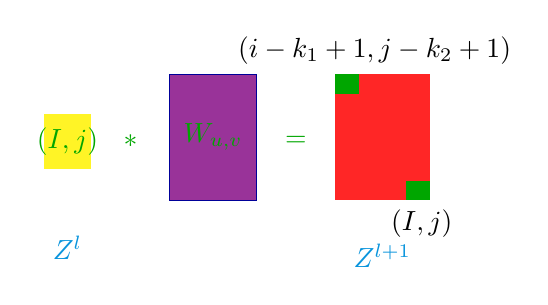
\begin{tikzpicture}[x=1cm,y=1cm]
\fill[yellow!85] (0,.4) rectangle (.6,1.1);\node[green!65!black] at (.3,.75) {$(I,j)$};
\node[green!65!black] at (1.1,.75) {$*$};
\filldraw[fill=violet!80,draw=blue!60!black] (1.6,0) rectangle (2.7,1.6);
\node[green!65!black] at (2.15,.8) {$W_{u,v}$};
\node[green!65!black] at (3.2,.75) {$=$};
\fill[red!85] (3.7,0) rectangle (4.9,1.6);
\fill[green!65!black] (3.7,1.35) rectangle (4,1.6);\fill[green!65!black] (4.6,0) rectangle (4.9,.25);
\node at (4.2,1.9) {$(i-k_1+1,j-k_2+1)$};\node at (4.8,-.3) {$(I,j)$};
\node[cyan!80!blue] at (.3,-.6) {$Z^l$};\node[cyan!80!blue] at (4.3,-.7) {$Z^{l+1}$};
\end{tikzpicture}
\origfig{10}{第 $l$ 个卷积层中像素 $(i,j)$ 与核卷积时，所影响的第 $(1+1)$ 个卷积层输出区域。}
\end{figure}

\begin{equation}
\begin{aligned}
\delta_{i,j}^l&=\frac{\partial E}{\partial z_p^l(i,j)}\\
&=\sum_{u=0}^{k_1-1}\sum_{v=0}^{k_2-1}\frac{\partial E}{\partial z_p^{l+1}(i-u,j-v)}\frac{\partial z_p^{l+1}(i-u,j-v)}{\partial z_p^l(i,j)}\\
&=\sum_{u=0}^{k_1-1}\sum_{v=0}^{k_2-1}\delta_p^{l+1}(i-u,j-v)\frac{\partial z_p^{l+1}(i-u,j-v)}{\partial z_p^l(i,j)}.
\end{aligned}\tag{6.123}
\end{equation}
根据式 (6.102)、(6.105)，有
\begin{equation}
\begin{aligned}
z_p^{l+1}(i-u,j-v)&=\sum_{m'=0}^{k_1-1}\sum_{n'=0}^{k_2-1}w_p^{l+1}(m',n')\sigma(z_p^l(i-u+m',j-v+n'))\\
&\quad+b_p^{l+1}.
\end{aligned}\tag{6.124}
\end{equation}
注意，
\begin{equation}
\frac{\partial\sigma(z_p^l(i-u+m',j-v+n'))}{\partial z_p^l(i,j)}=
\begin{cases}
\dfrac{\partial\sigma(z_p^l(i,j))}{\partial z_p^l(i,j)},&m'=u,\ n'=v,\\
0,&\text{其他情形}.
\end{cases}
\tag{6.125}
\end{equation}
将式 (6.125) 代入式 (6.124)，并利用链式法则，得到
\begin{equation}
\frac{\partial z_p^{l+1}(i-u,j-v)}{\partial z_p^l(i,j)}=w_p^{l+1}(u,v)\sigma'(z_p^l(i,j)).
\tag{6.126}
\end{equation}
将式 (6.126) 代入式 (6.123)，得到
\begin{equation}
\delta_{i,j}^l=\sum_{u=0}^{k_1-1}\sum_{v=0}^{k_2-1}\delta_p^{l+1}(i-u,j-v)w_p^{l+1}(u,v)\sigma'(z_p^l(i,j)).
\tag{6.127}
\end{equation}
若使用翻转后的核，式 (6.127) 可改写为
\begin{equation}
\begin{aligned}
\delta_{i,j}^l&=\operatorname{rot}_{180^0}\left\{\sum_{u=0}^{k_1-1}\sum_{v=0}^{k_2-1}\delta_p^{l+1}(i+u,j+v)w_p^{l+1}(u,v)\right\}\sigma'(z_p^l(i,j))\\
&=\delta_p^{l+1}(i,j)*\operatorname{rot}_{180^0}\{w_p^{l+1}(u,v)\}\sigma'(z_p^l(i,j)),
\end{aligned}\tag{6.128}
\end{equation}
其中，$*$ 表示卷积运算。
